\section{I$^2$GL Design}
\label{sec:approach}
In this section, we propose the design of I$^2$GL. We first give an overview of I$^2$GL, and then present technical details including graph construction, embedding and node classification.

%we are the first to analyze cryptocurrency transactions and solve the identity inferring problem based on graph deep learning.

\newcommand{\tabincell}[2]{\begin{tabular}{@{}#1@{}}#2\end{tabular}}
\begin{table}[!t]
  \centering
  \caption{NOTATIONS}
  \label{tab:notations}
  \begin{tabular}{ll}
    \\[-2mm]
    \hline
    \hline\\[-2mm]
    {\bf \small Symbol}&\qquad {\bf\small Meaning}\\
    \hline
    \vspace{1mm}\\[-3mm]
    \vspace{1mm}
    $G$      &   \tabincell{l}{The transaction graph}\\
    \vspace{1mm}
    $V$          &  \tabincell{l}{Set of nodes in the graph}\\
    \vspace{1mm}
    $E$          &  \tabincell{l}{Set of edges in the graph}\\
    \vspace{1mm}
    $Y$   &  \tabincell{l}{Embedding of the graph}\\
    \vspace{1mm}
    $\vec{y_i}$   &  \tabincell{l}{Embedding of the node $v_i$}\\
    \vspace{1mm}
    $(v_i,v_j,w,h,r)$  &   \tabincell{l}{Directed edge from node $v_i$ to $v_j$, with weight $w$, \\block height $h$ and relation $r$}\\
    \vspace{1mm}
    $E_{i}^{+}$   &  \tabincell{l}{Set of edges that point to node $v_i$}\\
    \vspace{1mm}
    $E_{i}^{-}$   &  \tabincell{l}{Set of edges that initiated from node $v_i$}\\
    \vspace{1mm}
    $X$    &	\tabincell{l}{Feature matrix of all nodes}\\
    \vspace{1mm}
    $\vec{x_i}$   &  \tabincell{l}{Feature vector of the node $v_i$}\\
    \vspace{1mm}
    $A^r,a^r_{ij}$    &	\tabincell{l}{Adjacency matrix of relation $r$, and the element \\is defined as first-order proximity between node $v_i$ \\and $v_j$}\\
    \vspace{1mm}
    $T^r,t^r_{ij}$    &	\tabincell{l}{Time-density matrix of relation $r$, and the element \\is defined as time variance of edges between node \\$v_i$ and $v_j$}\\
    \hline
    \hline
  \end{tabular}
\end{table}


\subsection{Overview}
\label{subsec:methodology}
%In I$^2$GL, identity inferring task is turned into node classification problem, simply, predicting the identity of accounts on a small sample of labeled accounts and the topology of the transaction graph.
The basic idea of I$^2$GL is to present the accounts in cryptocurrency and associated transactions as a graph. In the graph, accounts are represented as nodes with low dimensional vectors by embedding technique. Then, the identify inference is to classify nodes on the graph by given a labeled training set. Specifically, I$^2$GL consists of three phases: graph construction, graph embedding, and node classification, as shown in Fig.~\ref{fig:architecture}. The main notations used in this section are summarized in TABLE~\ref{tab:notations}.

\begin{figure*}
\centering
\begin{tikzpicture}[inner sep=1pt]
\node (log) at(0, 0) [label=above:{transaction logs}] {\tgelog{0.5}{0.1}};

\node [below=1 of log.south,anchor=north] (graph) [label=below:{transaction graph}]
{\tgegraph{0.7}};
\node[below=1 of graph.south, anchor=north] (desc) {\tgegraphdesc};

\node[right=1 of graph,anchor=west] (p2){\tgeparttwo{6}{gray!30}};
\node[above=1pt of p2.north,anchor=south] (p1){\tgepartone{5.7}};
\node[below=1pt of p2.south,anchor=north] (p3){\tgeparthree{6}{red!30}};

\node[eoa, right=1.3 of p2.east, anchor=west] (plus){+};

\node[rectlabel, right=0.5 of plus.east, anchor=west]
(relu){ReLU};

\node[right=0.5 of relu.east, anchor=west] (em) {\tgeebd{3}};

\node[rectlabel, below=0.5 of em.south, anchor=north]
(softmax){Softmax};

\node[below=0.7 of softmax.south, anchor=north] (ret) {\tgeret};


\draw[black, big arrow] (log.south) -- ($(graph.north) + (0, 4pt)$);

\draw[conn ] (graph.east) to [out=0,in=180] (p1.west);
\draw[conn ] (graph.east) to [out=0,in=180] (p2.west);
\draw[conn ] (graph.east) to [out=0,in=180] (p3.west);

\draw[conn ] (p1.east) to [out=0,in=180] (plus.west);
\draw[conn ] (p2.east) to [out=0,in=180] (plus.west);
\draw[conn ] (p3.east) to [out=0,in=180] (plus.west);

\draw[conn ] (plus.east) to [out=0,in=180] (relu.west);
\draw[conn ] (relu.east) to [out=0,in=180] (em.west);
\draw[conn ] (em.south) to [out=270,in=90] (softmax.north);
\draw[conn] (softmax.south) to (ret.north);
%\draw [decorate,thick, decoration={brace,amplitude=10pt, mirror}] (ri.west) --
%(ri.west|-rp.west);

\end{tikzpicture}
	\caption{Overall architecture.}
	\label{fig:architecture}
\end{figure*}


\textbf{Phase 1: Graph construction}. We construct the blockchain transaction graph as a directed graph $G=(V,E)$, where node $v \in V$ represents an account that can be an EOA or CA. We use the terms account and node interchangeably in the remainder of this paper. The total number of accounts is $N=|V|$.

The set $E$ contains edges, each of which can be represented as a quintuple, i.e., $E=\{(v_i,v_j,w,h,r)|v_i,v_j \in V, w\in \mathbb{R}^+ \cup\{0\}, h\in \mathbb{Z}, r\in R\}$, where $(v_{i},v_{j})$ indicates the direction of transaction (e.g., assets transfer or smart contract invocation) from $v_i$ to $v_j$, weight $w$ represents the amount of cryptocurrency, $h$ is the block height of transactions, and $r$ is a relation type which is detailed in the following sub-section.

%Analogously, the number of edges in ETG is represented as $|E|$.

\textbf{Phase 2: Graph embedding}.
Graph embedding provides an effective yet efficient way to solve the graph analytics problem~\cite{cai2018comprehensive}. The embedding process can be defined as follows: given $G=(V,E)$, we represent each node $v_{i}$ in a low-dimensional vector space $\vec{y_i}$. Based on such vectors (represented as a matrix $Y$), node classification can then be computed efficiently with high accuracy.

Typical network embedding techniques, such as random-walk based and deep learning based models, use the pure network structure to map into the embedding space~\cite{goyal2018capturing}. Our model is primarily motivated as an extension of GCNs (Graph Convolutional Networks)~\cite{kipf2016semi,schlichtkrull2018modeling}, which expand the convolution operator onto the non-Euclid graph structural space, and show effectiveness for entity classification in large-scale relational data.

\textbf{Phase 3: Node classification}.
The final objective of I$^2$GL is to predict account identities on the transaction graph. Given a labeled account set, supervised or semi-supervised methods can be used for entities classification. An intuitive way is simply stacking GCN layers of the form with a softmax ($\cdot$) activation on the output of the last layer~\cite{schlichtkrull2018modeling}. A loss function, such as cross-entropy error function, can be used as the objective in training.

Last but not least, the categorization is important to the performance of classification. For cryptocurrencies that support smart contracts, such as Ethereum, we propose a coarse taxonomy illustrated in TABLE~\ref{table:identity}, whose details will be presented in Section \ref{sec:experiments}.

 %To be frank, the perfect categorization does not exist because Ethereum and Ethereum-like blockchains are still in a development stage. \textcolor{red}{For accounts in Ethereum, we propose} a coarse but effective taxonomy.

\subsection{Graph Construction}
The transaction graph can be constructed based on original transaction records synchronized from the blockchain. In I$^2$GL, the graph is represented as three kinds of matrices: (a) \emph{account representations}, (b) \emph{adjacency matrices}, and (c) \emph{time density matrices}.


%(1) a node representation matrix that captures the structural and additional information of accounts, (2) a list of adjacency matrices which describe different relations, and (3) a list of time-density matrices that represent transaction intensiveness between each pair of nodes.

%Different from other studies~\cite{kipf2016semi,schlichtkrull2018modeling}, the graph is translated into

\paragraph{Account representations} To encode the overall structural and additional information of accounts, we denote the account representations as a feature matrix $X \in \mathbb{R}^{N \times d}$, where each account is depicted as $\vec{x_i}$ containing the following $d$ pre-defined features.

\begin{itemize}
	\item \emph{in-degree}: the number of incoming edges of a node, that is, the number of transactions pointing to an account. The in-degree of node $v_i$ can be counted as $|E_{i}^{+}|$, and $E_{i}^{+}=\{(v_j,v_i,w,h,r)| \forall v_j \in V\}$.
	\item \emph{out-degree}: the number of outgoing edges of a node, that is, the number of transactions initiated by an account. The out-degree of node $v_i$ can be counted as $|E_{i}^{-}|$, and $E_{i}^{-}=\{(v_i,v_j,w,h,r)| \forall v_j \in V\}$.
	\item \emph{weighted in-degree}: the sum of values of incoming edges of a node, which represents the total amount of cryptocurrencies received by an account. The weighted in-degree of node $v_i$ is $\sum_{e\in E_{i}^{+}}w$.
	\item \emph{weighted out-degree}: the sum of values of edges outgoing to a node, which represents the total amount of cryptocurrencies sent from an account. The weighted out-degree of node $v_i$ can be computed as $\sum_{e\in E_{i}^{-}}w$.
	%\item eccentricity
	%\item clustering coefficient
	\item \emph{account type}: whether the account is a smart contract or normal one.
\end{itemize}

\paragraph{Adjacency matrices} Different from social networks, edges in the transaction graph stand for heterogeneous activities such as money transfer, contract creation, and contract invocation. Obviously, such %multi-relations can not be measured in a uniform weighted model.
activitities should be represented as different edge types instead of being measured in uniform weighted graph.

To address the challenge, we divide the raw transaction graph into several sub-graphs and capture the relations of graph neighboring nodes using adjacent matrices. The set of adjacency matrices, $\{A^1,A^2,\dots,A^R|A^r\in \mathbb{R}^{N \times N}\}$, describes $R$ relations among $N$ nodes in the transaction graph. It is conceivable that the strategy of division has a large influence on classification performance.

In I$^2$GL, four major types of transactions are considered, including (I) \texttt{CALL} transactions with weight $w>0$, (II) \texttt{CALL} transactions with weight $w=0$, (III) \texttt{CREATION} transactions and (IV) \texttt{REWARD} transactions, which represent the relations of cryptocurrency transferring, smart contract invocation, smart contract deployment and mining rewarding, respectively \textcolor{red}{in usual}. More specifically, a transaction is regarded as type I if an account transfer some ETH (cryptocurrency in Ethereum) to another one. And the ERC-20 token transferring transactions are regarded as type II since they are contract invocation without any ETH.

On one hand, for types II, III and IV, we calculate the frequency of repeated edges between a pair of nodes as the adjacent weight in the corresponding relation adjacent matrix. For cryptocurrency transferring, on the other hand, it is not sensible to use the assets amount directly as the adjacent weight. That is because the accounts have varied enormously in terms of cryptocurrency transferring which will lead to underflow and overflow in the process of training.

 Taking Ethereum transactions as an example, the amount of assets transferring is discretized into three ranges: (1) small transfers whose transaction values are less than 1 ETH (the cryptocurrency used in Ethereum); (2) medium transfers with transaction values between 1 ETH and 10 ETH; and (3) large transfers whose transaction values are more than 10 ETH. Then the ETH transferring matrix can be calculated in a similar way with other relations.

%forward transactions introduced above and 4 reverse relations in order to pass information from the opposite direction. Besides, a self loop as a special relation type is included to retain information of the previous layer in the GCN network.

%Specially, the adjacent matrices are modified to preserve the asymmetric proximity of transaction graph, which will be addressed in detail later.

\paragraph{Time-density matrices}
Note that $a^r_{ij}$ in adjacent matrix $A^r$ indicates the number of edges belonging to relation $r$ between nodes $v_i$ and $v_j$.
In fact, more information could be exploited on transaction graphs. Within each block, transactions are labeled with block heights which can be regarded as timestamps. These repeated edges are located at different time intervals along the time axis. Based on such information, we expand on these adjacent features to open a new dimension.


\begin{figure}[htbp]
\centering
\begin{tabular}{c}
	\subfigure[Time variance histogram of all nodes.]{
		\label{fig:high_order}
		%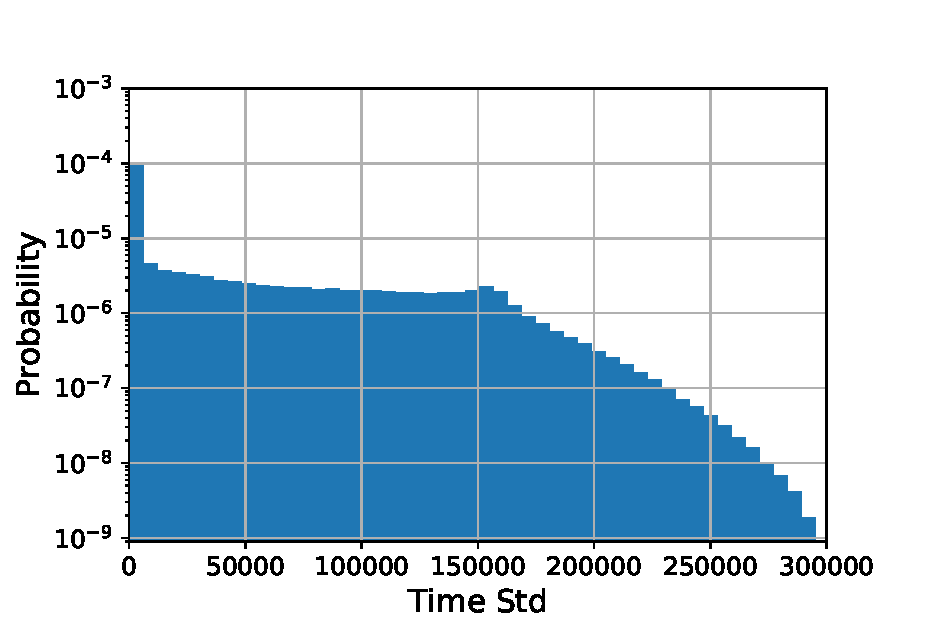
\includegraphics[width=0.22\textwidth]{fig/all_time_std_pdf.eps}
    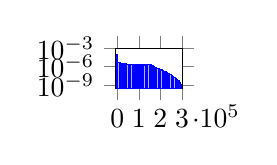
\begin{tikzpicture}
\begin{axis}[ymax=0.001,ybar,ymode=log,bar width=6023.807139652907,log origin=infty,xmin=-6023.807139652907,ytick align=outside,enlargelimits=0,
width=.20\textwidth,
every x tick scale label/.style={at={(xticklabel cs:1)},anchor=south west},
]
\addplot  plot coordinates {
(0.0, 9.451382865223466e-05)
(6023.807139652907, 5.4237855234498505e-06)
(12047.614279305813, 4.160561994558263e-06)
(18071.421418958722, 3.567714777734051e-06)
(24095.228558611627, 3.385128656276782e-06)
(30119.03569826453, 3.165308635083816e-06)
(36142.842837917444, 2.9615307529739165e-06)
(42166.64997757035, 2.6626153921894407e-06)
(48190.45711722325, 2.5490152149843527e-06)
(54214.26425687616, 2.3890921746281617e-06)
(60238.07139652906, 2.275444535473124e-06)
(66261.87853618198, 2.248248838151831e-06)
(72285.68567583489, 2.156718467673447e-06)
(78309.49281548779, 2.138350693042835e-06)
(84333.2999551407, 2.0591366985764506e-06)
(90357.1070947936, 2.0862137410228693e-06)
(96380.9142344465, 2.0135969575995206e-06)
(102404.72137409942, 2.000948347937872e-06)
(108428.52851375232, 1.9544830989369192e-06)
(114452.33565340523, 1.9188391745245435e-06)
(120476.14279305813, 1.8834088288869425e-06)
(126499.94993271104, 1.8642104701322076e-06)
(132523.75707236395, 1.8633324240581345e-06)
(138547.56421201685, 1.8347365992133192e-06)
(144571.37135166978, 1.9392715439779758e-06)
(150595.17849132267, 2.1352419353211166e-06)
(156618.98563097557, 2.1487685910568386e-06)
(162642.79277062847, 1.6649889352174985e-06)
(168666.5999102814, 1.0367825656806102e-06)
(174690.4070499343, 7.939434987619423e-07)
(180714.2141895872, 6.496829018892185e-07)
(186738.02132924012, 5.151757357311993e-07)
(192761.828468893, 4.3131047016972446e-07)
(198785.6356085459, 3.5105231280444205e-07)
(204809.44274819884, 2.852225882239295e-07)
(210833.24988785174, 2.272003544101756e-07)
(216857.05702750463, 1.7961974958539996e-07)
(222880.86416715756, 1.4827113164349042e-07)
(228904.67130681046, 1.1445449230418602e-07)
(234928.47844646336, 8.545524088479658e-08)
(240952.28558611625, 6.371766780774196e-08)
(246976.09272576918, 4.777045262457526e-08)
(252999.89986542208, 3.780344313509607e-08)
(259023.70700507498, 2.6009148572545693e-08)
(265047.5141447279, 1.8557622430411254e-08)
(271071.3212843808, 1.31232291611476e-08)
(277095.1284240337, 8.305841241232658e-09)
(283118.9355636866, 5.624241069063257e-09)
(289142.74270333955, 2.7053311471443514e-09)
(295166.54984299245, 1.3526655735721757e-09)
(301190.35698264535, 3.0850267467435584e-10)
};\end{axis}
\end{tikzpicture}

	%\caption{Example of a high-order proximity caption.}
	}\\
	\subfigure[Time variance histogram of Phish/Hack nodes.]{
		\label{fig:asymmetric}
		%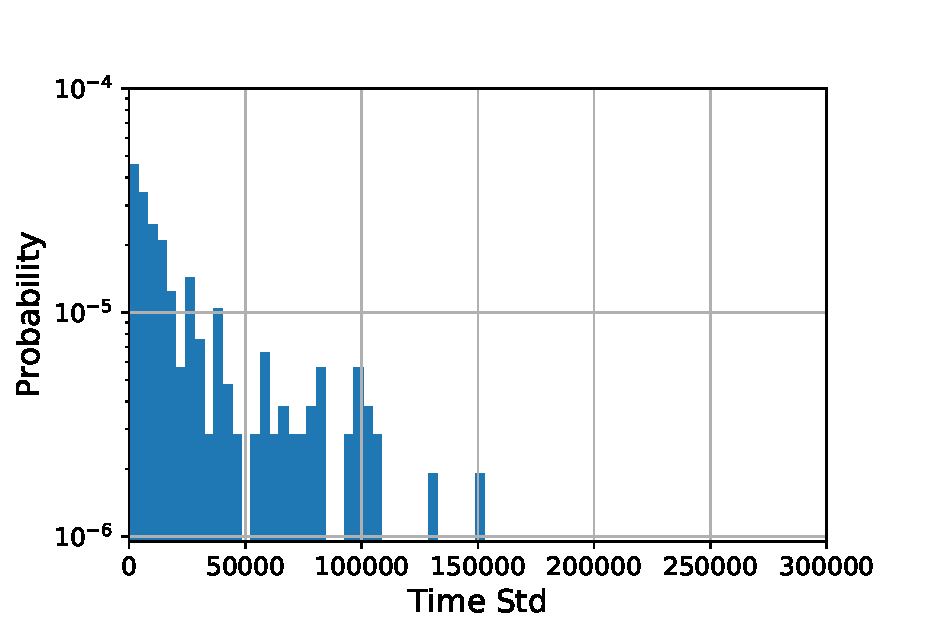
\includegraphics[width=0.22\textwidth]{fig/fake_time_std_pdf.eps}
    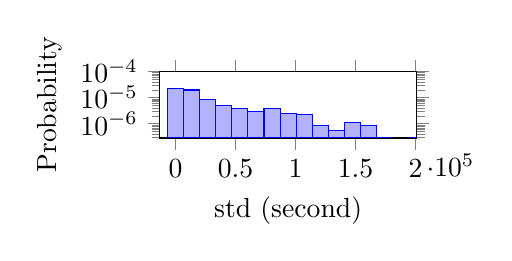
\begin{tikzpicture}
\begin{axis}[ymax=0.0001,ybar,ymode=log,bar width=13410.783587930588,log origin=infty,xmin=-13410.783587930588,ytick align=outside,enlargelimits=0,
width=.40\textwidth,
height=.20\textwidth,
ylabel=Probability,
xlabel=std (second),
every x tick scale label/.style={at={(xticklabel cs:1)},anchor=south west},
]
\addplot  plot coordinates {
(0.0, 2.1630081044550223e-05)
(13410.783587930588, 1.9637836737815332e-05)
(26821.567175861175, 8.822796215540222e-06)
(40232.350763791765, 5.122913931604e-06)
(53643.13435172235, 3.699882283936222e-06)
(67053.91793965294, 2.8460632953355556e-06)
(80464.70152758353, 3.984488613469778e-06)
(93875.48511551411, 2.561456965802e-06)
(107286.2687034447, 2.2768506362684445e-06)
(120697.0522913753, 8.538189886006666e-07)
(134107.83587930587, 5.692126590671111e-07)
(147518.61946723645, 1.1384253181342222e-06)
(160929.40305516706, 8.538189886006666e-07)
(174340.18664309764, 2.8460632953355556e-07)
(187750.97023102822, 0.0)
(201161.75381895882, 2.8460632953355556e-07)
};\end{axis}
\end{tikzpicture}

	}
\end{tabular}
\caption{Time variance histogram of accounts in Ethereum.}
\label{fig:time_std}
\end{figure}

%Fig.~\ref{fig:time_std} illustrates the distribution of time variance when transaction happens of whole accounts and hack \& phish accounts in Ethereum. 
\textcolor{red}{As shown in Fig.~\ref{fig:time_std},} we observe that the time variance distribution of Phish/Hack accounts is more concentrated compared with other accounts, because they are more active in a short period. This observation inspires us to exploit transaction time information to increase inference performance.

To describe time-density information, we use a set of matrices $\{T^1,T^2,\dots,T^R|T^r\in \mathbb{R}^{N \times N}\}$. Given a sequence $\{h_{ij1}^r,h_{ij2}^r,\dots,h_{ijm}^r | h_{ijk}^r>0\}$ as the block height of $m$ transactions in relation $r$ between node $v_i$ and $v_j$, the time-density of each relation $r$ is computed as%Equation \ref{eq:time}

\begin{equation}
t_{ij}^r=g\Bigg(\sqrt{Var\Big[\frac{1}{m}\sum_{k=1}^m h_{ijk}^r\Big]}\Bigg)
\label{eq:time}
\end{equation}

\noindent where $g(\cdot)$ is the function of squash which can be logarithmic function.

\subsection{Embedding}
\label{sec:rGCN layers}
Based on the above matrices, we propose a multi-layer Graph Convolutional Network with the following layer-wise propagation rule:

%The method can be understood as a more abstract propagation rule:
\begin{equation}
H^{(l+1)}=\delta(\sum_{r\in R} (T^r\odot (D^r)^{-1}A^r)H^{(l)}W_r^{(l)}),\forall r
\end{equation}

\noindent where $H^{(l)}$ is the matrix of activations of the $l$-th layer, and here the $0$ layer is set as the account representations, that is, $H^{(0)}=X$. We use $\delta(\cdot)$ to denote an activation function such as the ReLU$(\cdot)$ = max$(0,\cdot)$. Note that $A^r$ is the adjacent matrix of relation $r$, and $D^r$ is a diagonal matrix of relation $r$ where $d^r_{ii}=\sum_{j}a^r_{ij}$. The symbol $\odot$ indicates point-wise multiplication.

The edge weight $a^r_{ij}$ in adjacency matrix $A^r$ is defined as the \emph{first-order proximity}~\cite{tang2015line} which represents similarity between nodes $v_i$ and $v_j$. Further, the \emph{second-order proximity} evaluates the similarity of two nodes by comparing their neighborhood~\cite{goyal2018graph}. In the cryptocurrency transaction graph, we find that second-order proximity also plays an important role in preserving the local structure. As shown in Figure \ref{fig:high_order}, nodes $v_a$ and $v_c$ are smart contracts and node $v_b$ is a normal user. Obviously, $v_a$ is not adjacent to $v_c$  but they have a similar neighbor structure. First-order proximity may miss the similarity of nodes that are separated far away, but second-order proximity can capture this similarity.

We feed the input into a GCN model with 2 hidden layers, as a trade-off between preserving second-order proximity and introducing noise. The input of the $l$-th layer is $H^{(l)}=\{h_1^{(l)},h_2^{(l)},...,h_N^{(l)}|h_i^{(l)}\in \mathbb{R}^{N \times d^{(l)}}\}$. Hence, the method can be treated as a special case of the forward updating process as

\begin{equation}
h_i^{(l+1)}=\delta(\sum_{r\in R} \sum_{j \in N_i^r} \frac{t_{ij}^r}{\hat c_{i,r}}W_r^{(l)}h_j^{(l)})
\end{equation}

\noindent where $h_i^{(l)}$ is the hidden state of node $v_i$ in the $l$-th layer of the neural network, $r \in R$ represents a kind of relation, $N_i^r$ denotes the set of neighbors of node $v_i$ under relation $r$, and $t_{ij}^r$ is the time-density of transactions from node $v_i$ to $v_j$, which is represented in Eq.~(\ref{eq:time}). $\hat c_{i,r}$ is normalization coefficient. 


\begin{figure}[htbp]
	\centering
	\subfigure[Second-order proximity]{
		\label{fig:high_order}
    \begin{tikzpicture}
\tikzset{
  base/.style={draw, on grid, align=center, minimum height=2.5ex},
  pn/.style={base, circle},
}


\tikzmath{\r=1.5;}

\node [pn] (a) at (0, 0) {};
\node at (a) {\footnotesize a};
\node [pn] (b) at (\r, 0) {};
\node at (b) {\footnotesize b};
\node [pn] (c) at (2*\r, 0) {};
\node at (c) {\footnotesize c};

\node[pn] (a1) at ({\r*cos(60)}, {\r*sin(60)}) {};
\node[pn] (a2) at ({\r*cos(120)}, {\r*sin(120)}) {};
\node[pn] (a3) at ({\r*cos(180)}, {\r*sin(180)}) {};
\node[pn] (a4) at ({\r*cos(240)}, {\r*sin(240)}) {};
\node[pn] (a5) at ({\r*cos(300)}, {\r*sin(300)}) {};

\node[pn] (b1) at ({2*\r + \r*cos(60)}, {\r*sin(60)}) {};
\node[pn] (b2) at ({2*\r + \r*cos(120)}, {\r*sin(120)}) {};
\node[pn] (b3) at ({2*\r + \r*cos(0)}, {\r*sin(0)}) {};
\node[pn] (b4) at ({2*\r + \r*cos(240)}, {\r*sin(240)}) {};
\node[pn] (b5) at ({2*\r + \r*cos(300)}, {\r*sin(300)}) {};

\draw[->, >=stealth] (a1)-- (a);
\draw[->, >=stealth] (a2) -- (a);
\draw[->, >=stealth] (a3) -- (a);
\draw[->, >=stealth] (a4) -- (a);
\draw[->, >=stealth] (a5) -- (a);

\draw[->, >=stealth] (b1) -- (c);
\draw[->, >=stealth] (b2) -- (c);
\draw[->, >=stealth] (b3) -- (c);
\draw[->, >=stealth] (b4) -- (c);
\draw[->, >=stealth] (b5) -- (c);

\draw[->, >=stealth] (b) -- (a) node [midway, above] {\tiny invocation};
\draw[->, >=stealth] (b) -- (c) node [midway, above] {\tiny invocation};
\end{tikzpicture}

		%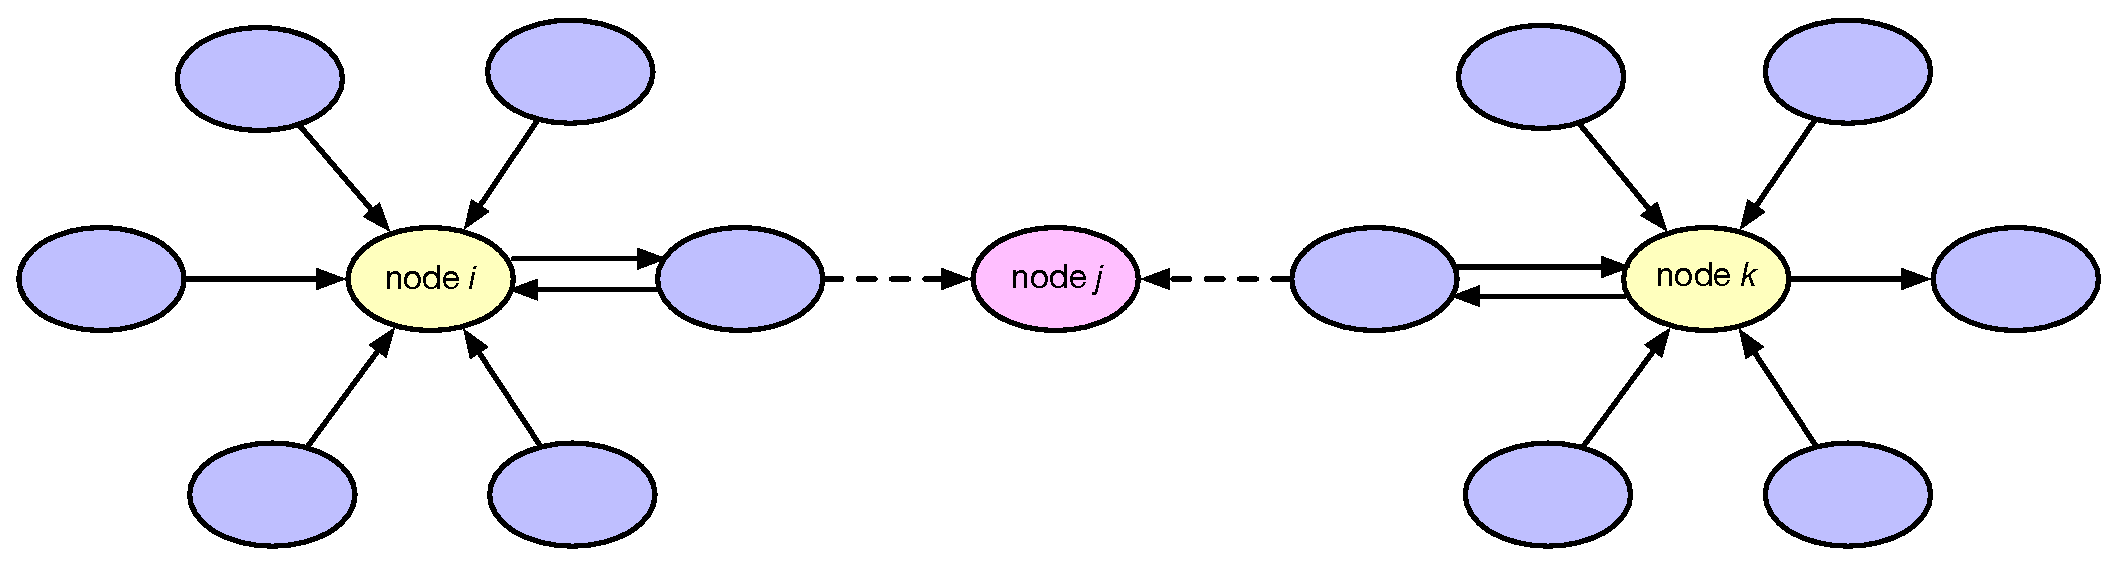
\includegraphics[width=2.0in]{fig/high_order_proximity.eps}
	%\caption{Example of a high-order proximity caption.}
	}
	\subfigure[Asymmetric proximity]{
		\label{fig:asymmetric}
    \begin{tikzpicture}
\tikzset{
  base/.style={draw, on grid, align=center, minimum height=2.5ex},
  pn/.style={base, circle},
}


\tikzmath{\r=1.0;}

\node [pn] (a) at (0, 0) {};
\node at (a) {\footnotesize a};
\node [pn] (b) at (\r, 0) {};
\node at (b) {\footnotesize b};
\node [pn] (c) at (2*\r, 0) {};
\node at (c) {\footnotesize c};

%\node[pn] (a1) at ({\r*cos(60)}, {\r*sin(60)}) {};
%\node[pn] (a2) at ({\r*cos(120)}, {\r*sin(120)}) {};
%\node[pn] (a3) at ({\r*cos(180)}, {\r*sin(180)}) {};
%\node[pn] (a4) at ({\r*cos(240)}, {\r*sin(240)}) {};
%\node[pn] (a5) at ({\r*cos(300)}, {\r*sin(300)}) {};

\node[pn] (b1) at ({2*\r + \r*cos(360.0/14)}, {\r*sin(360.0/14)}) {};
\node[pn] (b2) at ({2*\r + \r*cos(360.0*3/14)}, {\r*sin(360.0*3/14)}) {};
\node[pn] (b3) at ({2*\r + \r*cos(360.0*5/14)}, {\r*sin(360.0*5/14)}) {};
\node[pn] (b4) at ({2*\r + \r*cos(360.0*9/14)}, {\r*sin(360.0*9/14)}) {};
\node[pn] (b5) at ({2*\r + \r*cos(360.0*11/14)}, {\r*sin(360.0*11/14)}) {};
\node[pn] (b6) at ({2*\r + \r*cos(360.0*13/14)}, {\r*sin(360.0*13/14)}) {};

%\draw[->, >=stealth] (a1)-- (a);
%\draw[->, >=stealth] (a2) -- (a);
%\draw[->, >=stealth] (a3) -- (a);
%\draw[->, >=stealth] (a4) -- (a);
%\draw[->, >=stealth] (a5) -- (a);

\draw[->, >=stealth] (b1) -- (c);
\draw[->, >=stealth] (c) -- (b2);
\draw[->, >=stealth] (b3) -- (c);
\draw[->, >=stealth] (c) -- (b4);
\draw[->, >=stealth] (b5) -- (c);
\draw[->, >=stealth] (c) -- (b6);

\draw[->, >=stealth] (a) -- (b) node [midway, above] {\tiny deposit};
\draw[->, >=stealth] (b) -- (c) node  {};
\draw[->, >=stealth] (c) to [out=205, in=335]  node [midway, below] {\tiny
withdrawal}  (a);
\end{tikzpicture}

		%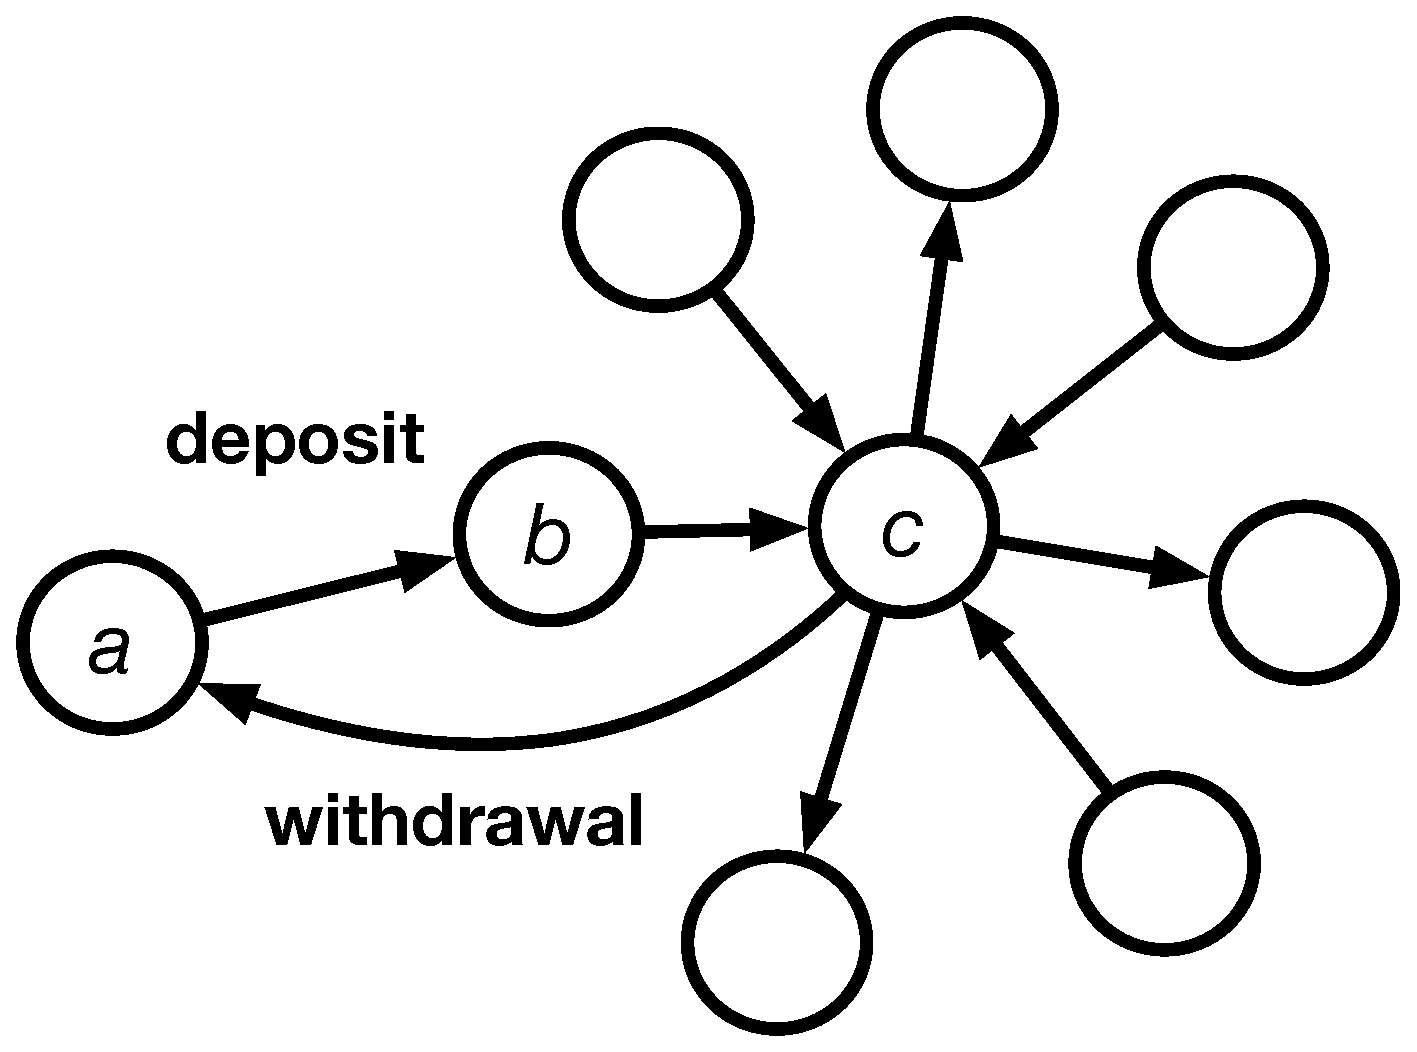
\includegraphics[width=1.5in]{fig/asymmetric.eps}
	}
	\caption{Examples of second-order and asymmetric proximity.}

\end{figure}


Another overlooked closeness, \emph{asymmetric proximity} should also be preserved in the transaction graph. For instance, as shown in Fig. \ref{fig:asymmetric}, suppose node $v_a$ is cryptocurrency trader, and node $v_b$ and $v_c$ are cryptocurrency exchange accounts. Consequently, edge $(v_a,v_b)$ stands for a deposit process and edge $(v_c,v_a)$ is a withdrawal process. Generally, edge weight can be $w^r_{ab}=w^r_{bc}=w^r_{ca}$ since deposit and withdrawal come in pairs in symmetric model. However, the proximity $(v_a,v_c)$ is not equal to proximity $(v_c,v_a)$ due to their asymmetric local structures.

Different from the asymmetric proximity preserving approach based on random walk~\cite{zhou2017scalable}, I$^2$GL use a non-probability graph embedding model. To preserve the asymmetric proximity, the coefficient $\hat c_{i,r}$ is introduced as:

\begin{equation}
\hat c_{i,r}=\frac{1}{g(d_i^r)\cdot |N_i^r|}
\end{equation}

\noindent where $d_i^r=\sum_{j}a^r_{ij}$, $g$ is a squash function, and $|N_i^r|$ is used for normalization.



\subsection{Node Classification}
We use the cross-entropy loss function as the training objective:
\begin{equation}
L=-\sum_{i=1}^T\sum_{j=1}^m y_{i,j}\log p_{i,j}+\lambda ||\theta||^2
\end{equation}
where $T$ is the number of training samples, $y_{i,j}$ is the true probability of node $v_i$ belonging to category $j$, $\theta$ is the set of all parameters and $\lambda$ is the coefficient for $L_2$  regularization. The output of the last GCN layer is a probability matrix $P=\{\vec{p_1},\vec{p_2},...,\vec{p_N}|\vec{p_i}\in \mathbb{R}^{1 \times m}\}$, where $\vec{p_i}$ describes the probability of classifying node $v_i$ into $m$ categories.
